\documentclass[11pt, journal]{IEEEtran}

\usepackage{lipsum}
\usepackage[T1]{fontenc}
\usepackage{fouriernc}
\usepackage{cases}
\usepackage{amsmath}
\usepackage{amssymb}
\usepackage[noadjust]{cite}
\usepackage{hyperref}
\usepackage{multirow}
\usepackage{graphicx}
\usepackage{adjustbox}
\usepackage{makecell}
\usepackage[dvipsnames]{xcolor}
\usepackage{tikz}
\usepackage{lipsum}
\usepackage{listings}
\usepackage{fontawesome5}
\usepackage{tcolorbox}
\usepackage[dvipsnames]{xcolor}
\usepackage[ruled]{algorithm2e}
\usepackage{array}
%\usepackage{caption}
\usepackage{bibtex}
\usepackage{cite}

%\addbibresource{bibliography.bib}

\hypersetup{
    colorlinks=true,
    linkcolor=blue,
    anchorcolor=blue,
    urlcolor=blue,
    citecolor=blue
}

\definecolor{codeCOMMENT}{HTML}{649541}
\definecolor{codeSTRING}{HTML}{37864A}
\definecolor{codeKEY}{HTML}{C678DD}
\definecolor{codeFUNC}{HTML}{61AFEF}
\definecolor{codeVALUES}{HTML}{C69438}

\newcommand{\eq}{\; = \;}
\newcommand{\nwl}{

\vspace{11pt}

}
\newcommand{\centered}[2]{\begin{tabular}{#1} #2 \end{tabular}}

\lstdefinestyle{standstyle}{
    commentstyle=\color{codeCOMMENT},
    keywordstyle=\bfseries\color{codeKEY},
    numberstyle=\scriptsize\ttfamily\color{codeVALUES},
    stringstyle=\color{codeSTRING},
    basicstyle=\ttfamily\linespread{1}\scriptsize\color{black!80},
    breakatwhitespace=false,
    breaklines=true,
    captionpos=b,
    keepspaces=true,
    numbers=left,
    numbersep=5pt,
    showspaces=false,
    showstringspaces=false,
    showtabs=false,
    tabsize=4,
    xleftmargin=15pt,
}

\lstset{style=standstyle}

%\newfloat{Code}{htbp}{loa}

\DeclareMathAlphabet{\mathcal}{OMS}{zplm}{m}{n}
\DeclareMathOperator*{\argmax}{arg\,max}
\DeclareMathOperator*{\argmin}{arg\,min}

\newcommand{\norm}[1]{\left\lVert#1\right\rVert}
\newcommand\commentalg[1]{\textcolor{ForestGreen}{{\footnotesize #1}}}
\SetCommentSty{commentalg}

\title{$k$-means is (\textit{really}) all you need}
\author{Leonardo Biason ($2045751$) \quad Alessandro Romania ($2046144$)}

\begin{document}

\maketitle

\begin{abstract}
    The $k$-means algorithm is a well known clustering algorithm, which is often used in unsupervised learning settings. However, the algorithm requires to perform multiple times the same operation on the data, and it can greatly benefit from a parallel implementation, so that to maximize the throughput and reduce computation times. With this project, we propose some possible implementations, based on some libraries that are considered to be the \text{de-facto} standard when it comes to writing multithreaded or parallel code, and we will discuss also the results of such implementations
\end{abstract}

\begin{keywords}
    Sapienza, ACSAI, Multicore Programming
\end{keywords}
\nwl
\begin{tcolorbox}[colback = Purple!20, colframe = Purple!40]
    \begin{center}
        \faIcon{github} Check our repository \href{https://www.github.com/ElBi21/PSEM-kmeans}{on GitHub}
        \verb|ElBi21/PSEM-kmeans|
    \end{center}
\end{tcolorbox}

\section{Introduction}

When talking about clustering and unsupervised learning, it's quite common to hear about the $k$-means algorithm, and for good reasons: it allows to efficiently cluster a dataset of $d$ dimensions, and it employs the notion of convergence in order to do so. This, computationally speaking, means to repeat some operations over and over again until some stopping conditions are met.
\nwl
The algorithm is not perfect though, and presents some issues:
\begin{itemize}
    \item [1)] the algorithm is fast in clustering, but we cannot be certain that it clusters \textit{well};
    \item [2)] the algorithm doesn't work with non-linear clusters;
    \item [3)] the initialization can make a great impact in the final result.
\end{itemize}
\nwl
Many people prefer to use other clustering methods, such as the fitting of Gaussian Mixture Models. Albeit not being perfect, $k$-means still works well in simple, linear clusters. For the sake of this project, we are going to consider a vanilla $k$-means algorithm with Lloyd's initialization (the first $k$ centroids will be selected randomly).

\subsection{Algorithm structure}

The $k$-means algorithm can be described with the following pseudocode, where $X$ is the set of data points, $C = \{\mu_1, \; \mu_2, \; ..., \; \mu_k \}$ is the set of centroids and $Y$ is the set of assignments:

\begin{algorithm}
    \label{algkmeans}
    \LinesNumbered
    \tcp{Initialize the centroids}
    \For{$k$ in $[1, \; |C|]$}{
        $\mu_k \gets \text{a random location in the input space}$
    }
    \BlankLine
    \While{$\text{convergence hasn't been reached}$}{
        \tcp{Assign each point to a cluster}
        \For{$i$ in $[1, \; |X|]$}{
            $y_i \gets \argmin_k \left(\norm{\mu_k - x_i}\right)$ 
        }
        \BlankLine
        \tcp{Compute the new position of each centroid}
        \For{$k$ in $[1, \; |C|]$}{
            $\mu_k \gets \textsc{Mean}(\{ \; x_n : z_n = k \; \})$
        }
    }
    \tcp{Return the centroids}
    \Return $Y$

    \caption{$k$-means (Lloyd's initialization)}
\end{algorithm}

The algorithm consists of 4 main blocks:
\begin{itemize}
    \item the \textbf{initialization block}, where all the centroids will receive a starting, random position (as per Lloyd's method);
    \item the \textbf{assignment block}, where the Euclidean distance between a point and all centroids is computed, for all centroids. The point will be assigned to a cluster depending on the following operation:
    \[ \argmin_k \left(\norm{\mu_k - x_i}\right) \]

    \item the \textbf{update block}, where the position of the centroids is updated, and the new position of a centroid $\mu_k$ is equal to the mean of all the data points positions belonging to cluster $k$
\end{itemize}

\subsection{Sequential Code Bottlenecks}

For implementing the $k$-means algorithm, we will base all the codebase upon the project made from professors Diego García-Álvarez and Arturo Gonzalez-Escribano from the University of Valladolid \cite{kmeans-univallo}. The code shown in this subsection is taken from their project, although slightly adapted for giving enough context in the code snippets.
\nwl
We described before the overall structure of the $k$-means algorithm: we will now proceed to examine its two main bottlenecks. As we can see from Algorithm \ref{algkmeans}, we have two main blocks that may cause performance issues: the \textbf{assignment block} and the \textbf{update block}.
\nwl
The first \textbf{for} block in the \textbf{initialization step} does not represent a major bottleneck, since it just needs to assign a random location to each of the $K$ centroids. It can be parallelized, but it won't help as much as parallelizing the two steps mentioned before.
\nwl
The second \textbf{for} block represents the \textbf{assignment step}, which is, unlike the initialization step, computationally expensive: for each point, the algorithm will have to compute the euclidean distance (here onwards denotes as $\ell_2$) between said point and all centroids $\mu_k \in C$, and select the lowest distance. This will determine the cluster of the point. In a C program, this may be accomplished with the following piece of code:
\nwl
\begin{lstlisting}[language = C]
int cluster;
// For each point...
for(i = 0; i < points_number; i++) {
    class = 1;
    minDist = FLT_MAX;
    // For each cluster...
    for(j = 0; j < K; j++) {
        // Compute the distance
        dist = l2_norm(&data[i*samples], &centroids[j*samples], samples);

        // If the distance is the lowest so far, replace it
        if(dist < minDist) {
            minDist = dist;
            class = j+1;
        }
    }
    
    // If the class is different from before, add a change to the counter
    if(classMap[i] != class) {
        changes++;
    }

    classMap[i]=class;
}\end{lstlisting}

Notice the presence of the two nested \textbf{for} loops: sequentially, they would take a time of $O(|X| \cdot |C|)$, which may be optimized just by taking a simple single instruction multiple data approach (indeed, with $m > 1$ different processes or threads, it would take a time of $O\left(\frac{|X| \cdot |C|}{m}\right)$ each, which is already better than the first option).
\nwl
The third \textbf{for} loop represents the update step, which also is computationally expensive: we would need to perform the mean of the coordinates of all the points belonging to a cluster $\mu_k$. This implies that all the coordinates of the points must be first summed, and then averaged on the number of points being classified to $\mu_k$. An implementation in the C language would look like the following:
\nwl
\begin{lstlisting}[language = C]
// For each point...
for (i = 0; i < lines; i++) {
    point_class = classMap[i];
    // Add 1 to the points classified for class k
    pointsPerClass[point_class - 1] += 1;

    // For each dimension...
    for(j = 0; j < samples; j++) {
        // ...add it to a table for summing and averaging
        auxCentroids[(point_class - 1) * samples + j] += data[i * samples + j];
    }
}

for (i = 0; i < K; i++) {
    for (j = 0; j < samples; j++) {
        // Average all dimensions
        auxCentroids[i * samples + j] /= pointsPerClass[i];
    }
}

maxDist = FLT_MIN;
for (i = 0; i < K; i++) {
    // Compute the moving distance, as a convergence check
    distCentroids[i] = euclideanDistance(&centroids[i * samples], &auxCentroids[i * samples], samples);
    if (distCentroids[i] > maxDist) {
        maxDist = distCentroids[i];
    }
}\end{lstlisting}


\section{Parallelizing with MPI}

\begin{figure}
    \label{mpi_speedup}
    \centering
    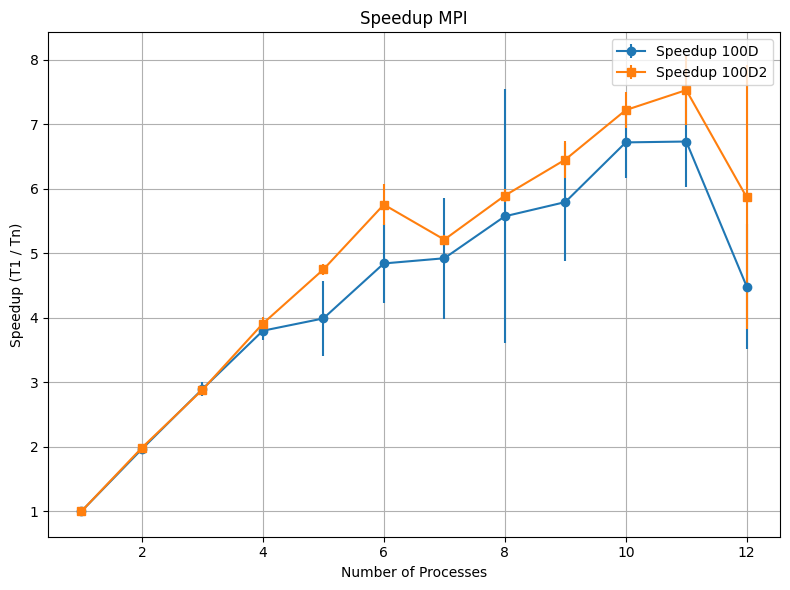
\includegraphics[width=\linewidth]{imgs/mpi_speedup.png}
    \caption{Speedup of the MPI application with three different tests}
\end{figure}

% TO REDO COMPLETELY

\section{Parallelizing with PThread}

\begin{figure}
    \label{pt_speedup}
    \centering
    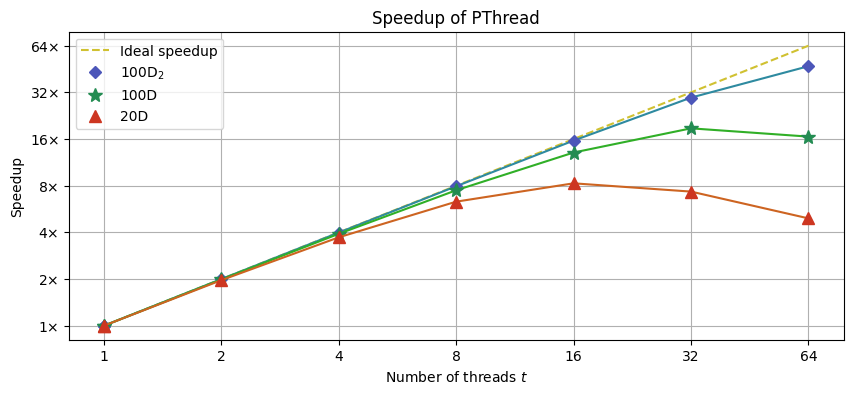
\includegraphics[width=\linewidth]{imgs/pt_speedup.png}
    \caption{Speedup of the PThread application with three different tests}
\end{figure}

% TO DO

\section{Parallelizing with CUDA}

In recent years, we have seen how GPUs play crucial roles when it comes to parallelizing a program with multiple threads. Indeed, the model proposed by NVIDIA for its CUDA platforms (namely, the Single-Thread Multiple-Data model) turned out to be very efficient, by allowing notable speed-ups and augmentation of the throughput. Here follows an explanation of how we decided to design a possible CUDA implementation.

\subsection{Designing the parallel structure}

As we have shown in Algorithm \ref{algkmeans}, the $k$-means algorithm can be logically split into two steps: the assignment step and the update step. However, while logically this division may sound reasonable, it is not appropriate for the STMD model that NVIDIA has at the core of its devices. This is because of the needed data for the two steps: the assignment step needs to work only with the data points, but can be parallelized by splitting the data into multiple parts; the update step instead needs to work with both all the data and all the centroids, so parallelizing the step as a whole becomes quite hard.
\nwl
A simpler approach would be to split the update step in two parts, one that uses a fraction of the points, and the other that uses a fraction of the centroids. This would create in total three parallelization steps. However, the assignment step and the first part of the update step can be merged together, since they both need to work with part of the data. This is the reason why we decided to implement the program with two kernels, called respectively \verb|step_1_kernel| and \verb|step_2_kernel|, where the first kernel can be considered as points-based and the second kernel as centroids-based.

\subsection{Program parameters and custom \texttt{atomicMax}}

We decided to organize the threads in two dimensional blocks of $32 \times 32$ threads, and the blocks are instead organized in a one dimensional grid. The size of the grid depends on the called kernel: usually, we have that $|X| \gg |C|$, so it's pointless for CUDA to reserve a grid of threads for the centroids that has the same size of the grid of the points. Indeed, the grids' single dimensions are dynamic, and are computed as follows:

\[ \texttt{points\_grid\_size} \; = \; \frac{\left| X \right|}{32 \times 32} + 1 \]
\[ \texttt{centroids\_grid\_size} \; = \; \frac{k}{32 \times 32} + 1 \]

The program makes also use of a custom function, called \verb|custom_atomic_max()|. This function has been implemented because it allows us to perform an \verb|atomicMax()|-like function for \verb|float| numbers, which would not be normally possible with the built-it CUDA function. We here show the function as a whole:
\nwl
\begin{lstlisting}[language = C]
__device__ float custom_atomic_max(float* value_address, float val) {
    int* address_as_int = (int*) value_address;
    int old = *address_as_int, assumed;
    do {
        assumed = old;
        old = atomicCAS(address_as_int, assumed, __float_as_int(fmaxf(val, __int_as_float(assumed))));
    } while (assumed != old);
    return __int_as_float(old);
}\end{lstlisting}
\nwl
The idea of the function is that CUDA tries continuously to perform an \verb|atomicCAS()| operation, which in turns performs atomically the following check:
\begin{center}
    \scriptsize
    \verb|old_value == to_compare ? new_value : old_value|
\end{center}

The function will exit only when the value in the specified address is equal to the one that the program expects to be there, before performing the atomic transaction. This is important, so that to avoid that the function overwrites any unintentional value.

\subsection{Analysis of the kernels}

As we mentioned previously, we are making use of two kernels: \verb|step_1_kernel| and \verb|step_2_kernel|. In both kernels, all operations that act on the global memory are performed atomically, which avoid potential race conditions. We here show how both kernels work, alongsize their code snippets.
\nwl
The first kernel is called on all the data, and each point is assigned to a thread. First, a preliminary check is performed, to make sure that each thread is assigned to a valid point. While the \verb|if| statement may seem like a possible cause of warp divergence, it doesn't actually impact that much. Indeed, we would only discard part of the final block of kernels, while all the previous blocks are fully used.
\nwl
Then, each thread will compute the $\ell_2$ norm of each point for all centroids, and will store the class to which each point will be assigned into the \verb|class_int| variable. If a change from the previous class assignment is detected, the number of changes will increase. After that, each thread will proceed to sum the coordinates of its assigned point into the auxiliary centroids matrix. The coordinates will then be averaged in the second kernel.
\nwl
\begin{lstlisting}[language = C]
__global__ void step_1_kernel(float* data, float* centroids, int* points_per_class, float* aux_centroids, int* class_map, int* changes_return) {

// Compute global thread index
int thread_index = (blockIdx.y * gridDim.x * blockDim.x * blockDim.y) + (blockIdx.x * blockDim.x * blockDim.y) + (threadIdx.y * blockDim.x) + threadIdx.x;

if (thread_index < gpu_n) {
    int class_int = class_map[thread_index];
    float min_dist = FLT_MAX;
    
    // For each centroid...
    for (int centroid = 0; centroid < gpu_K; centroid++) {
        float distance = 0.0f;

        // Compute the euclidean distance
        euclideanDistance(&data[thread_index * gpu_d], &centroids[centroid * gpu_d], gpu_d, &distance);

        // If distance is smaller, replace the distance and assign new class
        if (distance < min_dist) {
            min_dist = distance;
            class_int = centroid + 1;
        }
    }

    // If the class is different, add one change and write new class
    if (class_map[thread_index] != class_int) {
        atomicAdd(changes_return, 1);
    }
    
    // Map the value to the class map
    class_map[thread_index] = class_int;

    int class_assignment = class_map[thread_index];
    int point_index = class_assignment - 1;

    atomicAdd(&(points_per_class[point_index]), 1);

    for (int dim = 0; dim < gpu_d; dim++) {
        int index = point_index * gpu_d + dim;
        atomicAdd(&aux_centroids[index], data[thread_index * gpu_d + dim]);
    }
}}\end{lstlisting}

The second kernel performs the same check as \verb|step_1_kernel| on each thread, to ensure that all threads are mapped to a valid centroid. After that, all threads will compute, for each dimension of the centroids, the average coordinate. Once computed, each thread will then perform the $\ell_2$ norm between the previous centroid and the new one, so that to compute the \verb|max_distance| variable, needed for convergence. Finally, via the use of the \verb|custom_atomic_max()| function, the gratest distance is stored in memory.
\nwl
\begin{lstlisting}[language = C]
__global__ void step_2_kernel(float* centroids_table, float* centroids, int* points_per_class, float* max_distance) {
// Index of the thread
int thread_index = (blockIdx.y * gridDim.x * blockDim.x * blockDim.y) + (blockIdx.x * blockDim.x * blockDim.y) +
                        (threadIdx.y * blockDim.x) +
                        threadIdx.x;

if (thread_index < gpu_K) {
    float distance;
    // For each dimension...
    for (int d = 0; d < gpu_d; d++) {
        centroids_table[thread_index * gpu_d + d] /= (float) points_per_class[thread_index];
        // Compute Euclidean distance (l_2 norm) to check for maximum distance
        distance += pow((centroids[thread_index * gpu_d + d] - centroids_table[thread_index * gpu_d + d]), 2);
    }

    // Perform sqrt of distance
    //distance = sqrt(distance);

    // Exchange atomically, disregard old value
    custom_atomic_max(max_distance, distance);
}}
\end{lstlisting}

After executing the second kernel, the program continues repeating in loop the two kernels until one of the convergence conditions is met.

\begin{figure*}
    \label{stats_mpi_omp}
    \centering
    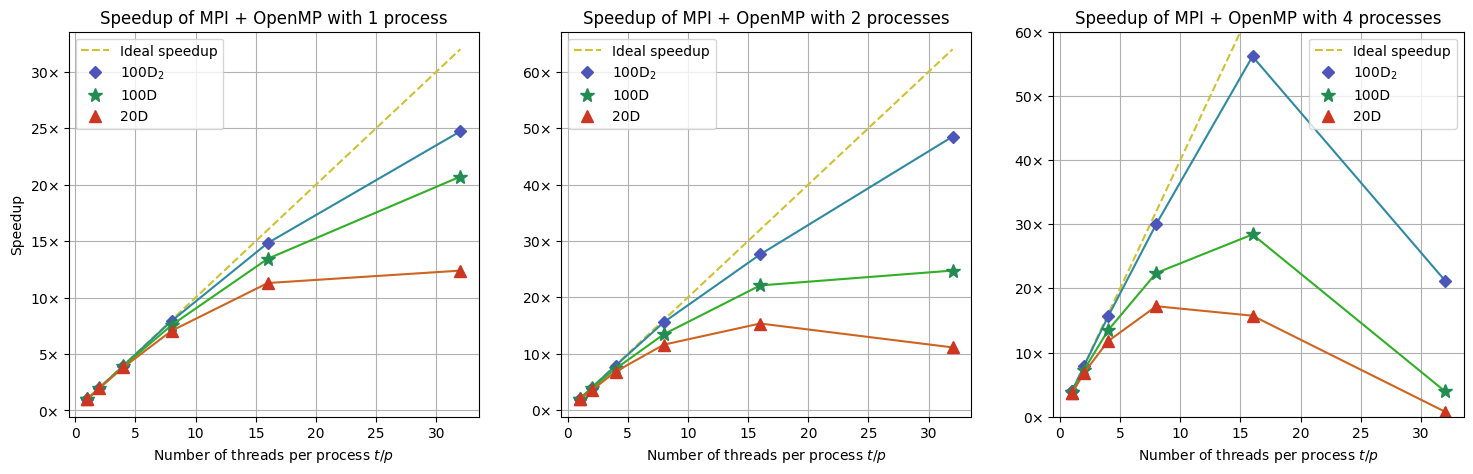
\includegraphics[width=\linewidth]{imgs/mpi_omp_speedup.png}

    \caption{Comparison of the speedup of the MPI + OpenMP program, on three different input tests. Each plot compares the program on a set amount of processes}
\end{figure*}

\section{Interlacing Multi-processing with Multi-threading with MPI + OpenMP}

So far, we implemented various solutions for our programs, which employed either multi-processing or multi-threading parallelism techniques, without using both approaches at the same time. However, these techniques are not mutually exclusive, and can be mixed together in order to achieve better performances. In fact, in high performance computing tasks, multi-process techniques are used within clusters to connect nodes and coordinate them, while multi-threading are used for performing computations, given the directives of the master process(es).
\nwl
In this section we will show how multi-threading approaches can be combined with the famous multi-processing library MPI, and this will be done thanks to the OpenMP library.

% TO REDO COMPLETELY

With MPI, we noticed that by augmenting the number of processes, the speed-up continued to grow. However, as expected, after a given number of processes we don't have anymore a linear scaling of the performances. With the input file \verb|input100D.inp|, which has $|X| = 10^4$, we start observing a non-linear increase already at $p = 5$, while with input file \verb|input100D2.inp|, which has $|X| = 10^5$, we stop increasing linearly after $p = 6$. We can see this behaviour in Figure \textbf{1}. This is because the overhead of exchanging data starts to become tangible, affecting negatively the performances. The parameters given to the program were the following:

\begin{center}
    \footnotesize
    \verb|<program> <input> 40 5000 1 000.1 <output>|
\end{center}

For the sole exception that with \verb|input2D2.inp| the number of centroids was $10$, as $|X_{2D}| = 20$.

Regarding the CUDA implementation, we show in Figure 2 its performances, compared to the ones of the sequential version. For this comparison, two different test inputs have been used, so that to better show the capabilities of this version. We can notice how the sequential version takes, in most of the cases, higher times for finishing executing. The only exception to this is with the input \verb|input2D2.inp|, where $|X|$ is incredibly small. In that case, there is a great overhead, given by the memory movements needed by CUDA.
\nwl
However, the difference can be seen with files containing a greater amount of data: the sequential version on input file \verb|input100D2.inp| takes large amount of data, with both of the tests. On Table \ref{cuda_seq_exec} are listed the average timings for both versions on 30 samples each, and as we can see, the advantage of using CUDA against the sequential counterpart becomes evident when the number of data gets over the order of $10^4$ (indeed, the input file \verb|input20D.inp| contains 10,000 points). At the end, CUDA is capable of reaching speedups of roughly $15.41\times$ over the sequential version:

\[ \frac{\frac{17.353409s}{1.171914s} + \frac{74.396411s}{4.647139s}}{2} \simeq 15.41 \]

\subsection{MPI + OpenMP}

\section{Conclusions}

% Bibliography
\bibliographystyle{plain}
\bibliography{bibliography}

\begin{table*}
    \renewcommand{\arraystretch}{1.3}
    \caption{Average execution times of MPI $\left(\mu \pm \sigma^2\right)$}
    \label{mpi_timings_table}
    \centering
    \begin{tabular}{|c||c|c|c|}
    \hline
    \multirow{2}{*}{\textbf{Processes}} & \multicolumn{3}{c|}{\textbf{Input files (in dimensions)}} \\\cline{2-4}
     & 20D & 100D & 100D$_2$ \\
    \hline\hline
    1 & 0.35482 $\pm$ 0.00039 & 1.06557 $\pm$ 0.00096 & 111.25387 $\pm$ 0.11351 \\
    \cline{2-4} 
    2 & 0.18259 $\pm$ 0.00432 & 0.53813 $\pm$ 0.00434 & 55.92949 $\pm$ 0.11749 \\
    \cline{2-4} 
    4 & 0.09535 $\pm$ 0.00171 & 0.27635 $\pm$ 0.00172 & 28.07182 $\pm$ 0.12835 \\
    \cline{2-4} 
    8 & 0.052 $\pm$ 0.00045 & 0.14474 $\pm$ 0.0007 & 14.08863 $\pm$ 0.05404 \\
    \cline{2-4} 
    16 & 0.03135 $\pm$ 0.00039 & 0.07982 $\pm$ 0.00039 & 7.10323 $\pm$ 0.02457 \\
    \cline{2-4} 
    32 & 0.02421 $\pm$ 0.00625 & 0.04941 $\pm$ 0.01561 & 3.63824 $\pm$ 0.01364 \\
    \cline{2-4} 
    64 & 0.04227 $\pm$ 0.00405 & 0.06498 $\pm$ 0.00777 & 2.06993 $\pm$ 0.01525 \\
    \hline
    \end{tabular}
\end{table*}

\begin{table*}
    \renewcommand{\arraystretch}{1.3}
    \caption{Average execution times of PThread $\left(\mu \pm \sigma^2\right)$}
    \label{pt_timings_table}
    \centering
    \begin{tabular}{|c||c|c|c|}
    \hline
    \multirow{2}{*}{\textbf{Threads}} & \multicolumn{3}{c|}{\textbf{Input files (in dimensions)}} \\\cline{2-4}
     & 20D & 100D & 100D$_2$ \\
    \hline\hline
    1 & 0.35589 $\pm$ 0.00116 & 1.07345 $\pm$ 0.00179 & 111.49448 $\pm$ 0.08208 \\
    \cline{2-4} 
    2 & 0.18134 $\pm$ 0.00051 & 0.5372 $\pm$ 0.00025 & 55.72216 $\pm$ 0.02585 \\
    \cline{2-4} 
    4 & 0.09344 $\pm$ 0.0002 & 0.27037 $\pm$ 0.00011 & 27.87802 $\pm$ 0.0107 \\
    \cline{2-4} 
    8 & 0.04993 $\pm$ 0.00015 & 0.13759 $\pm$ 0.000005 & 13.96211 $\pm$ 0.01513 \\
    \cline{2-4} 
    16 & 0.029 $\pm$ 0.00015 & 0.07174 $\pm$ 0.00024 & 7.01285 $\pm$ 0.00178 \\
    \cline{2-4} 
    32 & 0.01924 $\pm$ 0.00026 & 0.03934 $\pm$ 0.00015 & 3.5571 $\pm$ 0.00333 \\
    \cline{2-4} 
    64 & 0.01443 $\pm$ 0.00048 & 0.02464 $\pm$ 0.00028 & 1.87593 $\pm$ 0.00213 \\
    \hline
    \end{tabular}
\end{table*}

\begin{table*}
    \renewcommand{\arraystretch}{1.3}
    \caption{Average execution times of MPI + OpenMP $\left(\mu \pm \sigma^2\right)$}
    \label{mpi_omp_exec}
    \centering
    \begin{tabular}{|c|c||c|c|c|}
    \hline
    \multirow{2}{*}{\textbf{Processes}} & \multirow{2}{*}{\textbf{Threads}} & \multicolumn{3}{c|}{\textbf{Input files (in dimensions)}} \\\cline{3-5}
     & & 20D & 100D & 100D$_2$ \\
    \hline\hline
    \multirow{6}{*}{1} & 1 & 0.35709 $\pm$ 0.00048 & 1.06757 $\pm$ 0.0008 & 111.25387 $\pm$ 0.11351 \\
    \cline{2-5}
     & 2 & 0.18002 $\pm$ 0.0003 & 0.53609 $\pm$ 0.00047 & 55.93932 $\pm$ 0.0679 \\
    \cline{2-5}
     & 4 & 0.09277 $\pm$ 0.00033 & 0.27239 $\pm$ 0.00061 & 28.08522 $\pm$ 0.06347 \\
    \cline{2-5}
     & 8 & 0.05018 $\pm$ 0.00046 & 0.14105 $\pm$ 0.00067 & 14.04603 $\pm$ 0.02584 \\
    \cline{2-5}
     & 16 & 0.03136 $\pm$ 0.0005 & 0.07924 $\pm$ 0.00436 & 7.5028 $\pm$ 0.09568 \\
    \cline{2-5}
     & 32 & 0.02858 $\pm$ 0.00497 & 0.05141 $\pm$ 0.00269 & 4.50071 $\pm$ 0.18373 \\
    \hline\hline
    \multirow{6}{*}{2} & 1 & 0.18372 $\pm$ 0.00448 & 0.53968 $\pm$ 0.00436 & 55.92949 $\pm$ 0.11749 \\
    \cline{2-5} 
     & 2 & 0.1006 $\pm$ 0.02559 & 0.27507 $\pm$ 0.0028 & 28.04651 $\pm$ 0.06814 \\
    \cline{2-5} 
     & 4 & 0.05179 $\pm$ 0.001 & 0.14482 $\pm$ 0.00225 & 14.07429 $\pm$ 0.04251 \\
    \cline{2-5} 
     & 8 & 0.0305 $\pm$ 0.00054 & 0.0791 $\pm$ 0.00166 & 7.13597 $\pm$ 0.02573 \\
    \cline{2-5} 
     & 16 & 0.02306 $\pm$ 0.00071 & 0.04817 $\pm$ 0.00093 & 4.0312 $\pm$ 1.48805 \\
    \cline{2-5} 
     & 32 & 0.03185 $\pm$ 0.00557 & 0.04304 $\pm$ 0.0034 & 2.2939 $\pm$ 0.12168 \\
    \hline\hline
    \multirow{6}{*}{4} & 1 & 0.09674 $\pm$ 0.0014 & 0.27689 $\pm$ 0.00169 & 28.07182 $\pm$ 0.12835 \\
    \cline{2-5} 
     & 2 & 0.05165 $\pm$ 0.00107 & 0.14576 $\pm$ 0.00346 & 14.04567 $\pm$ 0.04577 \\
    \cline{2-5} 
     & 4 & 0.03005 $\pm$ 0.00056 & 0.07905 $\pm$ 0.00093 & 7.11934 $\pm$ 0.07096 \\
    \cline{2-5} 
     & 8 & 0.02056 $\pm$ 0.00046 & 0.04754 $\pm$ 0.00203 & 3.70751 $\pm$ 0.12491 \\
    \cline{2-5} 
     & 16 & 0.02249 $\pm$ 0.00256 & 0.03749 $\pm$ 0.00331 & 1.98168 $\pm$ 0.05976 \\
    \cline{2-5} 
     & 32 & 0.45262 $\pm$ 0.01723 & 0.26914 $\pm$ 0.00238 & 5.24488 $\pm$ 0.03644 \\
    \hline
    \end{tabular}
\end{table*}

\begin{table*}
    \label{mpi_pt_speedup_table}
    \centering
    \caption{Speedups of MPI and PThread}
    \renewcommand{\arraystretch}{1.3}
    \begin{tabular}{c c}
        \resizebox{0.45\textwidth}{!}{
        \begin{tabular}{|c||c|c|c|}
            \hline
            \multirow{2}{*}{\textbf{Processes}} & \multicolumn{3}{c|}{\textbf{Input files (in dimensions)}} \\
            \cline{2-4}
             & 20D & 100D & 100D$_2$ \\
            \hline\hline
            1 & 0.998$\times$ & 0.999$\times$ & 1.0$\times$ \\
            \cline{2-4}
            2 & 1.939$\times$ & 1.979$\times$ & 1.99$\times$ \\
            \cline{2-4}
            4 & 3.713$\times$ & 3.854$\times$ & 3.964$\times$ \\
            \cline{2-4}
            8 & 6.807$\times$ & 7.358$\times$ & 7.898$\times$ \\
            \cline{2-4}
            16 & 11.291$\times$ & 13.341$\times$ & 15.666$\times$ \\
            \cline{2-4}
            32 & 14.618$\times$ & 21.554$\times$ & 30.586$\times$ \\
            \cline{2-4}
            64 & 8.373$\times$ & 16.389$\times$ & 53.759$\times$ \\
            \hline
        \end{tabular}
    } & \resizebox{0.45\textwidth}{!}{
        \begin{tabular}{|c||c|c|c|}
            \hline
            \multirow{2}{*}{\textbf{Threads}} & \multicolumn{3}{c|}{\textbf{Input files (in dimensions)}} \\
            \cline{2-4}
            & 20D & 100D & 100D$_2$ \\
            \hline\hline
            1 & 0.995$\times$ & 0.992$\times$ & 0.998$\times$ \\
            \cline{2-4}
            2 & 1.952$\times$ & 1.982$\times$ & 1.997$\times$ \\
            \cline{2-4}
            4 & 3.788$\times$ & 3.939$\times$ & 3.992$\times$ \\
            \cline{2-4}
            8 & 7.089$\times$ & 7.74$\times$ & 7.97$\times$ \\
            \cline{2-4}
            16 & 12.206$\times$ & 14.845$\times$ & 15.868$\times$ \\
            \cline{2-4}
            32 & 18.395$\times$ & 27.07$\times$ & 31.283$\times$ \\
            \cline{2-4}
            64 & 24.537$\times$ & 43.226$\times$ & 59.319$\times$ \\
            \hline
        \end{tabular}
    }
    \end{tabular}
\end{table*}

\begin{table*}
    \label{mpi_omp_speedup_table}
    \centering
    \renewcommand{\arraystretch}{1.3}
    \caption{Speedups of MPI-OMP}
    \resizebox{0.45\textwidth}{!}{
        \begin{tabular}{|c|c||c|c|c|}
            \hline
            \multirow{2}{*}{\textbf{Processes}} & \multirow{2}{*}{\textbf{Threads}} & \multicolumn{3}{c|}{\textbf{Input files (in dimensions)}} \\
            \cline{3-5}
            & & 20D & 100D & 100D$_2$ \\
            \hline\hline
            \multirow{6}{*}{1} & 1 & 0.991$\times$ & 0.998$\times$ & 1.0$\times$ \\
            \cline{2-5}
             & 2 & 1.966$\times$ & 1.987$\times$ & 1.989$\times$ \\
            \cline{2-5}
             & 4 & 3.815$\times$ & 3.91$\times$ & 3.962$\times$ \\
            \cline{2-5}
             & 8 & 7.054$\times$ & 7.55$\times$ & 7.922$\times$ \\
            \cline{2-5}
             & 16 & 11.287$\times$ & 13.439$\times$ & 14.832$\times$ \\
            \cline{2-5}
             & 32 & 12.385$\times$ & 20.714$\times$ & 24.725$\times$ \\
            \hline\hline
            \multirow{6}{*}{2} & 1 & 1.927$\times$ & 1.973$\times$ & 1.99$\times$ \\
            \cline{2-5}
             & 2 & 3.519$\times$ & 3.872$\times$ & 3.968$\times$ \\
            \cline{2-5}
             & 4 & 6.835$\times$ & 7.354$\times$ & 7.907$\times$ \\
            \cline{2-5}
             & 8 & 11.606$\times$ & 13.463$\times$ & 15.594$\times$ \\
            \cline{2-5}
             & 16 & 15.353$\times$ & 22.109$\times$ & 27.604$\times$ \\
            \cline{2-5}
             & 32 & 11.114$\times$ & 24.745$\times$ & 48.511$\times$ \\
            \hline\hline
            \multirow{6}{*}{4} & 1 & 3.659$\times$ & 3.846$\times$ & 3.964$\times$ \\
            \cline{2-5}
             & 2 & 6.854$\times$ & 7.306$\times$ & 7.923$\times$ \\
            \cline{2-5}
             & 4 & 11.78$\times$ & 13.473$\times$ & 15.63$\times$ \\
            \cline{2-5}
             & 8 & 17.22$\times$ & 22.401$\times$ & 30.014$\times$ \\
            \cline{2-5}
             & 16 & 15.743$\times$ & 28.407$\times$ & 56.154$\times$ \\
            \cline{2-5}
             & 32 & 0.782$\times$ & 3.957$\times$ & 21.217$\times$ \\
            \hline
        \end{tabular}
    }
\end{table*}

\begin{table*}
    \renewcommand{\arraystretch}{1.3}
    \caption{Average execution times of CUDA and sequential versions}
    \label{cuda_seq_exec}
    \centering
    \begin{tabular}{|c|c||c|c|c|c|c|c|}
    \hline
    \multirow{2}{*}{\textbf{Test}} & \multirow{2}{*}{\textbf{Platform}} & \multicolumn{6}{|c|}{\textbf{Input files (in dimensions)}} \\\cline{3-8}
     & & 2D & 2D$_2$ & 10D & 20D & 100D & 100D$_2$ \\
    \hline\hline
    \multirow{2}{*}{\textbf{A}} & Sequential & 0.008275s & 0.000017s & 0.002507s & 0.106904s & 0.432722s & 17.353409s \\\cline{2-8}
     & CUDA & 0.000674s & 0.000129s & 0.001720s & 0.012662s & 0.055614s & 1.171914s \\
    \hline
    \multirow{2}{*}{\textbf{B}} & Sequential & 0.021466s & 0.000051s & 0.006098s & 0.232680s & 0.812164s & 74.396411s \\\cline{2-8}
     & CUDA & 0.002292s & 0.000151s & 0.002440s & 0.087071s & 0.055614s & 4.647139s \\
    \hline
    \end{tabular}
    \\
    \nwl
    \begin{tabular}{c c}
    \textbf{A}: \verb|<program> <input> 40 5000 1 0.0001 <output>| & \textbf{B}: \verb|<program> <input> 30 500 0.1 0.1 <output>|        
    \end{tabular}
\end{table*}

\end{document}